\documentclass[12pt]{article}

% This first part of the file is called the PREAMBLE. It includes
% customizations and command definitions. The preamble is everything
% between \documentclass and \begin{document}.

\usepackage[margin=1in]{geometry}  % set the margins to 1in on all sides
\usepackage{graphicx}              % to include figures
\usepackage{amsmath}               % great math stuff
\usepackage{amsfonts}              % for blackboard bold, etc
\usepackage{amsthm}                % better theorem environments
\usepackage{amssymb} 
\usepackage{mathptmx}
\usepackage{enumerate}
\usepackage{listings}
\usepackage{xcolor}
\usepackage{forest}
\usepackage{tabularx}  

% various theorems, numbered by section

\newtheorem{thm}{Theorem}[section]
\newtheorem{lem}[thm]{Lemma}
\newtheorem{prop}[thm]{Proposition}
\newtheorem{cor}[thm]{Corollary}
\newtheorem{conj}[thm]{Conjecture}
\newtheorem{mydef}[thm]{Definition}
\lstset{
	basicstyle          =   \sffamily,          
	keywordstyle        =   \bfseries,          
	commentstyle        =   \rmfamily\itshape,  
	stringstyle         =   \ttfamily,  
	flexiblecolumns,                
	numbers             =   left,   
	showspaces          =   false,  
	numberstyle         =   \fontsize{5}{skip},    
	showstringspaces    =   false,
	captionpos          =   t,      
	frame               =   lrtb,   
}

\lstdefinestyle{cpp}{
	language        =   cpp, 
	basicstyle      =   \fontsize{5}{skip},
	numberstyle     =   \fontsize{5}{skip},
	keywordstyle    =   \color{blue},
	keywordstyle    =   [2] \color{teal},
	stringstyle     =   \color{magenta},
	commentstyle    =   \color{red}\ttfamily,
	breaklines      =   true,   
	columns         =   fixed,  
	basewidth       =   0.5em,
}
\begin{document}


\title{ CSE 102 Spring 2021\\
	Homework Assignment 4}

\author{Jaden Liu \\ 
University of California at Santa Cruz\\
Santa Cruz, CA 95064 USA }

\maketitle


\section{HW4} 
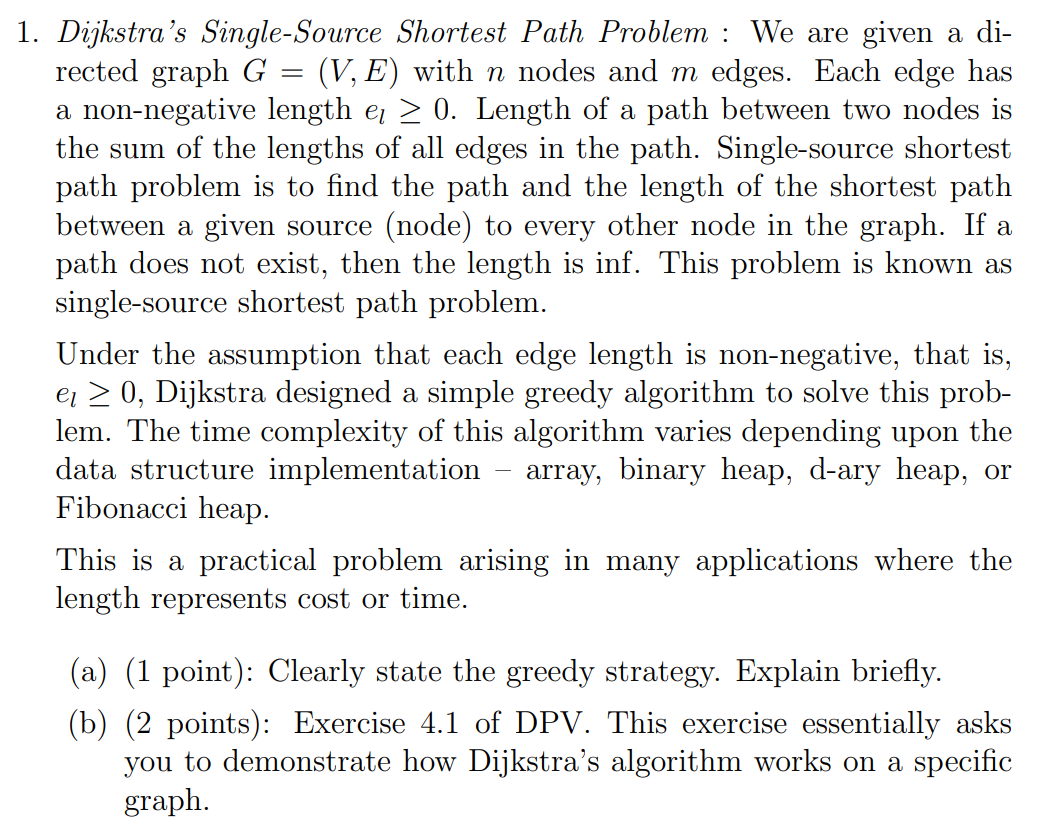
\includegraphics[scale=0.39]{1.png}
\begin{proof}[Solution for a]
	1. Find the minimum length node\\
	2. For the minimum length node, if there exist other shorter path to its neighbor nodes, then update the minimum length path.\\
	3. Keep the two steps and save the minimum until we reach the end node\\
	4. Calculate the minimum path.
\end{proof}
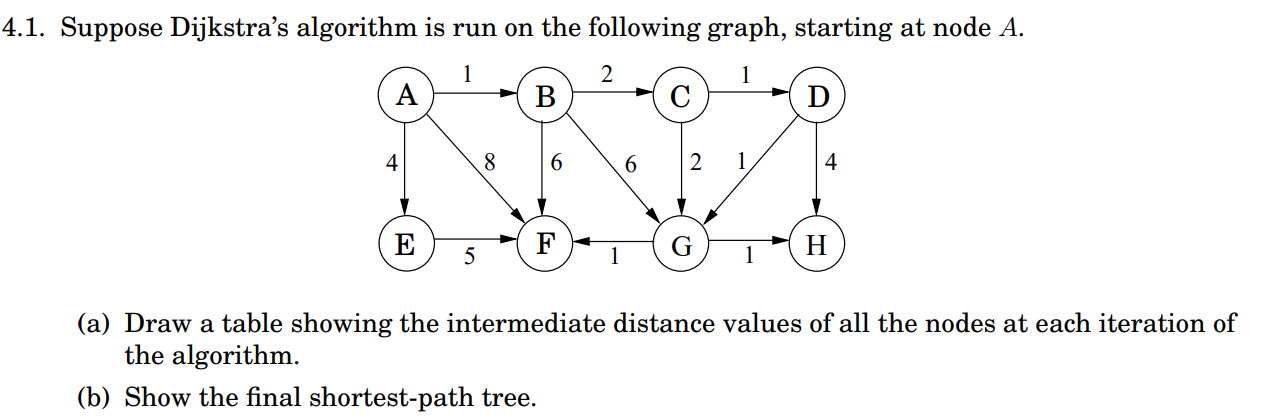
\includegraphics[scale=0.37]{1_1.png}
\begin{proof}[Solution for b]
    \begin{tabular}{rrrrrrrr}
	\multicolumn{1}{l}{A} & \multicolumn{1}{l}{B} & \multicolumn{1}{l}{C} & \multicolumn{1}{l}{D} & \multicolumn{1}{l}{E} & \multicolumn{1}{l}{F} & \multicolumn{1}{l}{G} & \multicolumn{1}{l}{H} \\
	0     & 1     & \multicolumn{1}{l}{\textcolor[rgb]{ .2,  .2,  .2}{$\infty$}} & \multicolumn{1}{l}{$\infty$} & 4     & 8     & \multicolumn{1}{l}{$\infty$} & \multicolumn{1}{l}{$\infty$} \\
	0     & 1     & 3     & \multicolumn{1}{l}{$\infty$} & 4     & 7     & 7     & \multicolumn{1}{l}{$\infty$} \\
	0     & 1     & 3     & 4     & 4     & 7     & 5     & \multicolumn{1}{l}{$\infty$} \\
	0     & 1     & 3     & 4     & 4     & 7     & 5     & 8 \\
	0     & 1     & 3     & 4     & 4     & 6     & 5     & 6 \\
\end{tabular}\\
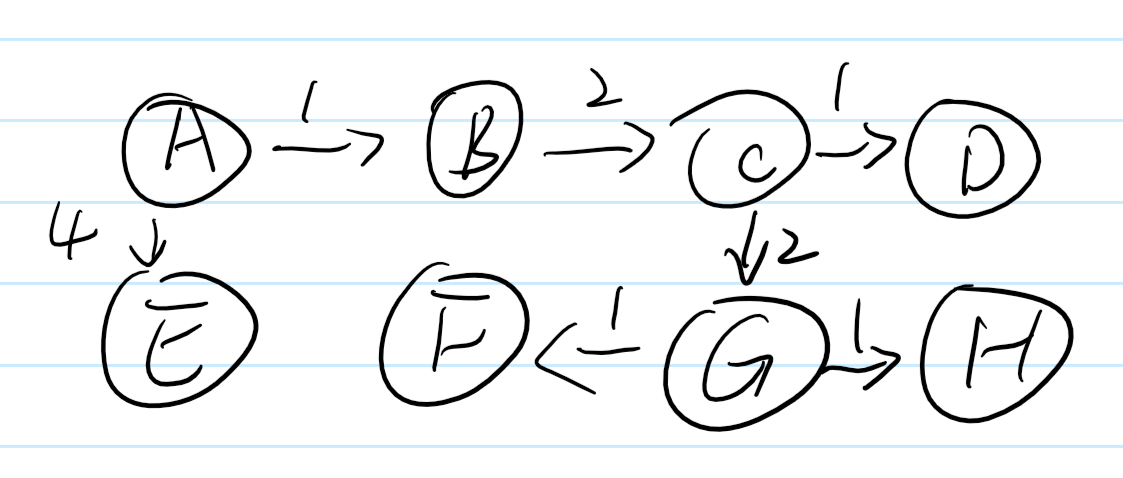
\includegraphics[scale=0.2]{1_9.png}
\end{proof}

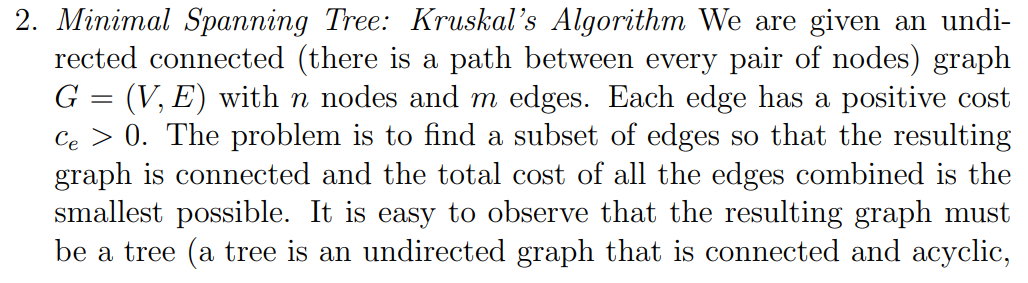
\includegraphics[scale=0.39]{2_1.png}\\
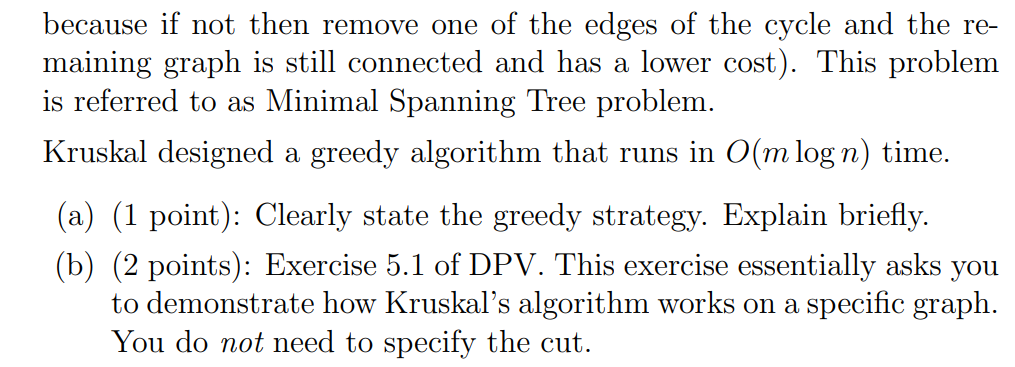
\includegraphics[scale=0.39]{2_2.png}
\begin{proof}[Solution for a]
	1. First sort all edges in the graph according to the edge value from small to large\\
	2. N vertices in a graph are regarded as a forest composed of n independent trees\\
	3. Select the edge according to the weight from small to large, the two vertices connected by the selected edge should belong to two different trees, then become an edge of the minimum spanning tree, and merge the two trees as one tree.\\
	4. Repeat (3) until all vertices are in a tree or have n-1 edges.
\end{proof}
\begin{proof}[Solution for b]
	\ \\
	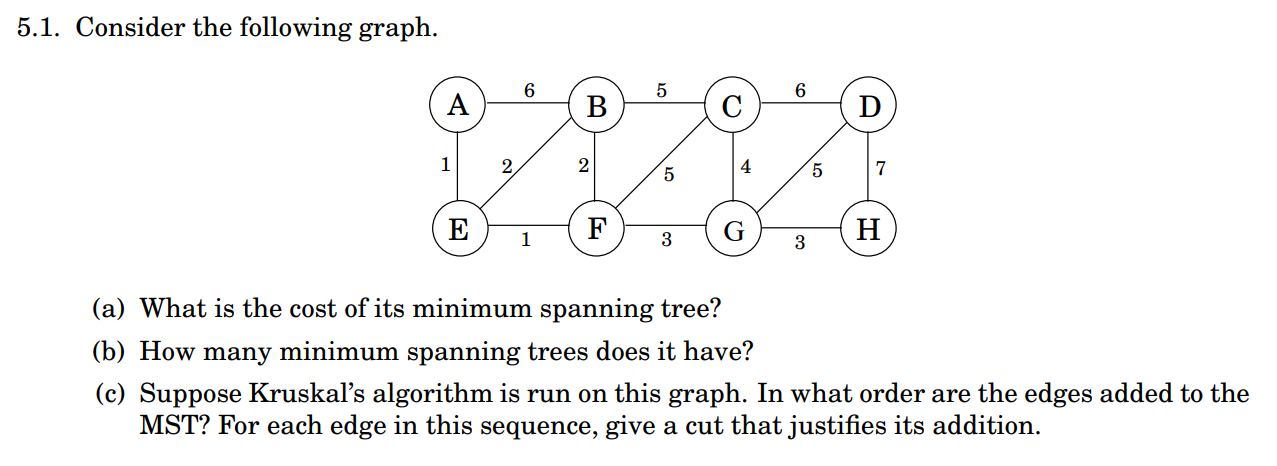
\includegraphics[scale=0.38]{2_3.png}
	(a)\\
	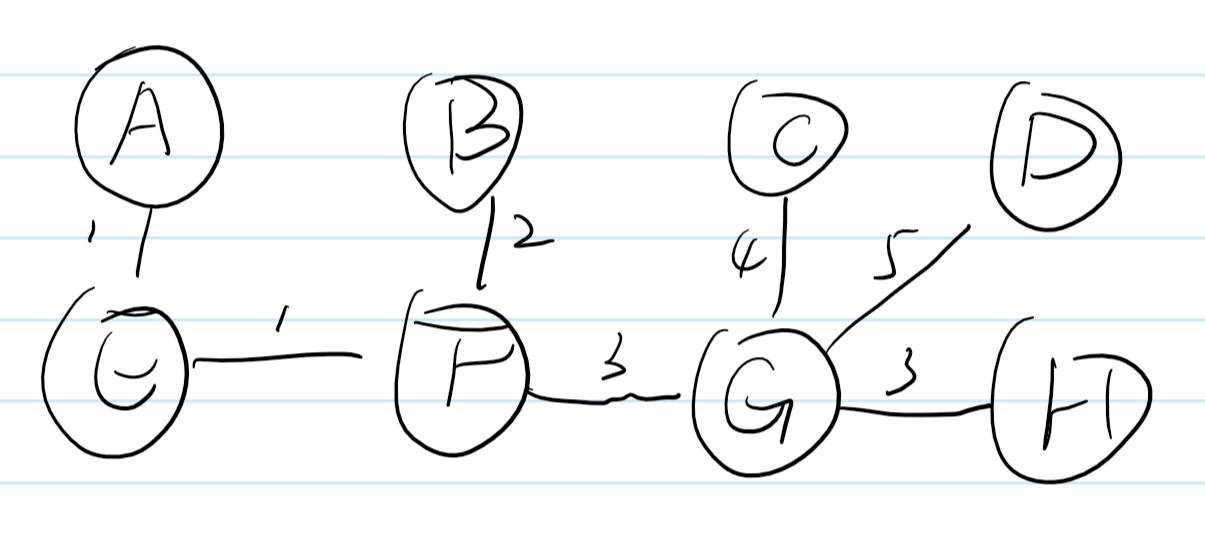
\includegraphics[scale=0.3]{2_4.png}\\
	(b)\\
	2\\
	(c)\\
	(A,E),(E,F)$->$(B,E)$->$(F,G),(G,H)$->$(G,C)$->$(G,D)
\end{proof}
\begin{proof}[Solution for a]
	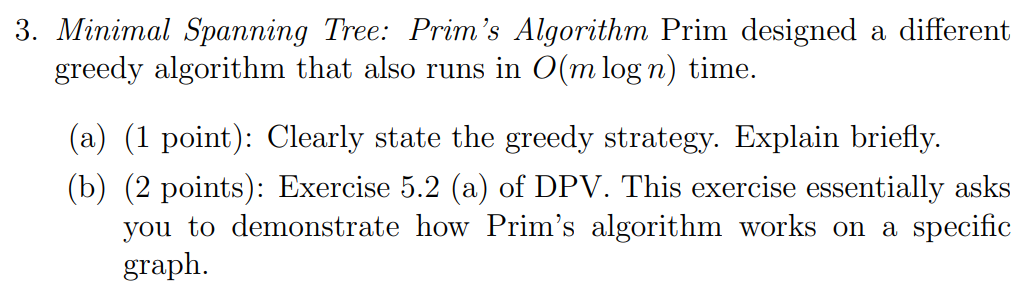
\includegraphics[scale=0.35]{3.png}\\
	1. First find the minimum length, absorb it into the minimal spanning tree.\\
	2. Find a minimum length that can generated by the set in the existing spanning tree, update it to the node attribute.\\
	3. Add the minimum length again and keep doing (1),(2) until we reach $n-1$ edges in tree or $n$ nodes.
\end{proof}
\begin{proof}[Solution for b]
	\ \\
	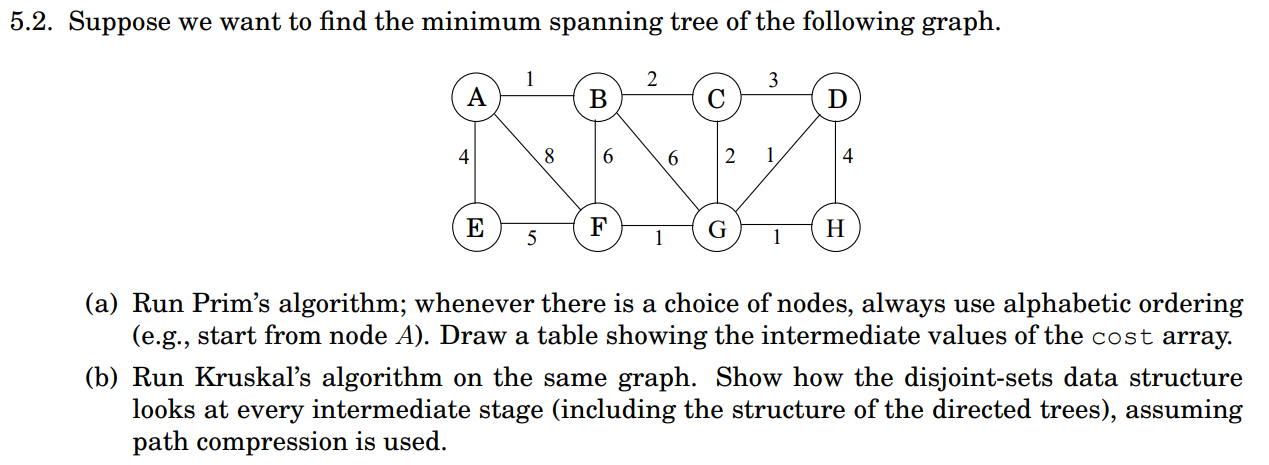
\includegraphics[scale=0.35]{3_2.png}\\
	(a)\\
    \begin{tabular}{llllllll}
	A    & B     & C   & D   & E    &F     & G     & H \\
	(A,0) & (A,1) & (A,$\infty$) & (A,$\infty$) & (A,4) & (A,8) & (A,$\infty$) & (A,$\infty$) \\
	(A,0) & (A,1) & (B,3) & (B,$\infty$) & (A,4) & (B,6) & (B,6) & (B,$\infty$) \\
	(A,0) & (A,1) & (B,3) & (C,3) & (A,4) & (B,6) & (C,2) & (C,$\infty$) \\
	(A,0) & (A,1) & (B,3) & (G,1) & (A,4) & (G,1) & (C,2) & (G,1) \\
	(A,0) & (A,1) & (B,3) & (G,1) & (A,4) & (G,1) & (C,2) & (G,1) \\
	(A,0) & (A,1) & (B,3) & (G,1) & (A,4) & (G,1) & (C,2) & (G,2) \\
	(A,0) & (A,1) & (B,3) & (G,1) & (A,4) & (G,1) & (C,2) & (G,2) \\
	(A,0) & (A,1) & (B,3) & (G,1) & (A,4) & (G,1) & (C,2) & (G,2) \\
\end{tabular}\\
    \begin{tabular}{lll}
	\textbf{vertex} & \textbf{edge}  & \textbf{cost} \\
	A     & N/A   & \multicolumn{1}{r}{0} \\
	B     & AB    & 0+1=1 \\
	C     & BC    & 1+2=3 \\
	G     & CG    & 3+2=5 \\
	D     & GD    & 5+1=6 \\
	F     & GF    & 6+1=7 \\
	H     & GH    & 7+1=8 \\
	E     & AE    & 8+4=12 \\
\end{tabular}%
(b)\\
(A,B),(F,G),(G,H)-$>$(B,C),(C,G)-$>$(C,D)-$>$(A,E)-$>$(E,F)
\end{proof}
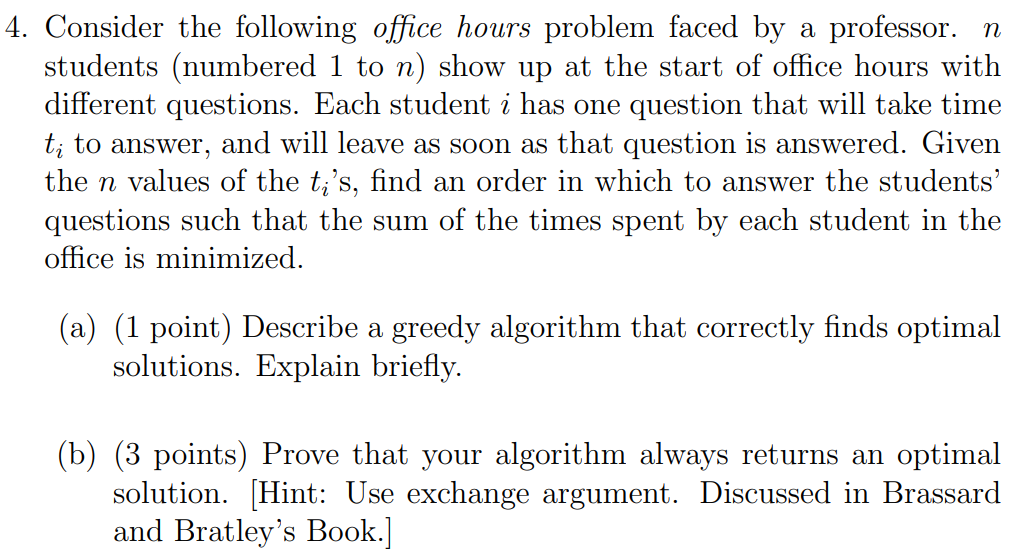
\includegraphics[scale=0.4]{4.png}\\
\begin{proof}[Solution for a]
	Sort students' list by their time to answer $t_i$. Keep answering students that needs smaller time until no more students has questions.
\end{proof}
\begin{proof}[Solution for b]
	\begin{align*}
		T(n)&=T(n-1)+t_1*n\\
		&=T(n-2)+t_1*n+t_2*(n-1)\\
		&\vdots
	\end{align*}
	From the equation, we can find that we can only minimize $t_i$ to get shorter time, since $n$ is a solid number to multiply. Therefore, it's faster that we solved shorter-time-consumed question, the shorter we have in the total time $T(n)$.
\end{proof}
\textbf{5.}\\
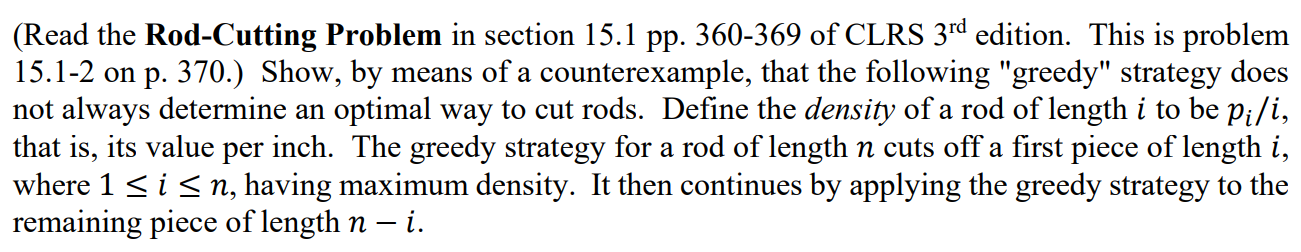
\includegraphics[scale=0.35]{5.png}\\
\begin{proof}[Solution]
	Using the sample example in section 15.1 of CLRS $3^{rd}$ edition:
	\centering
	    \begin{tabular}{lrrrrrrr}
		length i & 1     & 2     & 3     & 4     & 5     & 6     & 7 \\
		price $p_i$ & 1     & 5     & 8     & 9     & 10    & 17    & 17 \\
		density & 1     & 2.5   & 2.666666667 & 2.25  & 2     & 2.833333333 & 2.428571 \\
	\end{tabular}\\
	\raggedright
	For instance that we need to find the maximum price for a rod length n=4. By greedy algorithm that we will find that we first cut the maximum density, which is n=3, then the other part is not dividable anymore. We get the total price, which is 8+1=9.\\
	However, we can easily come up with that we cut the rod half then we get the maximum 5+5=10. Thus, there exist a counterexample.
\end{proof}
\textbf{6.}\\
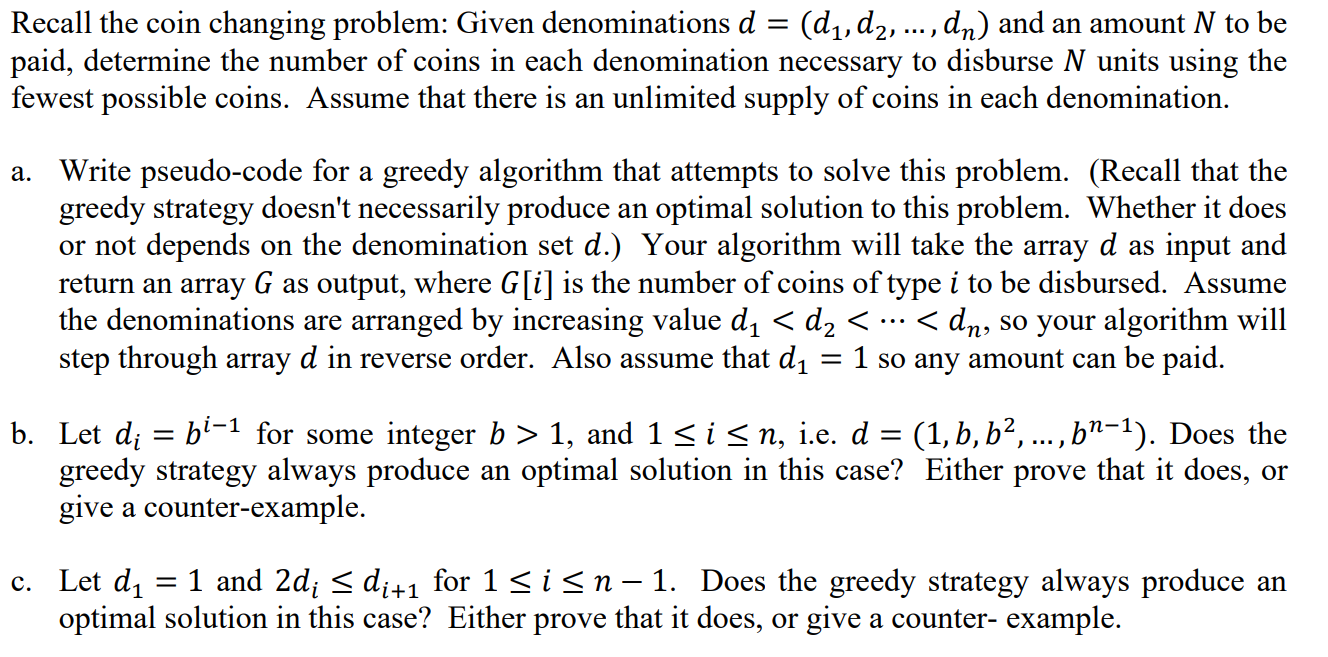
\includegraphics[scale=0.35]{6.png}\\
\begin{proof}[Solution for a]
	\begin{lstlisting}[language={python},numbers=left,numberstyle=\tiny,%frame=shadowbox,  
		rulesepcolor=\color{red!20!green!20!blue!20},  
		keywordstyle=\color{blue!70!black},  
		commentstyle=\color{blue!90!},  
		basicstyle=\ttfamily]  
		
	procedure(array d, amount N)
	result =[]
	N_copy,rem = N.copy() 
	for i in reversed(d): # reversed iteratet the input array 
				#so start from biggest one
		N_copy = rem
		coin_num = 0
		while(N_copy - i >= 0): # count for coin maximum 
					#coin we could use
			coin_num++
		rem = rem - coin_num*i
		result.append(coin_num)
	return result
	\end{lstlisting}
\end{proof}
\begin{proof}[Solution for b]
	The reason why greedy algorithm did not work well in general case is that if $d_i < d_{i-1} +d_{i-2}$, then we can subsitute amount of $d_i$ with smaller count with $d_{i-1}$ and $d_{i-2}$ combination. For this case, we have always $d_i > d_{i-1} +d_{i-2}$. Therefore, using greedy algorithm is in subset $d_i$, $d_{i-1}$, $d_{i-2}$,$\cdots$, $d_1$ is better than in subset $d_{i-1}, d_{i-2},\cdots, d_1$. Thus, this case alwasy produce an optimal solution.
\end{proof}
\begin{proof}[Solution for c]
	For this we have a counterexample that:\\
	\begin{tabular}{lrrr}
		& \multicolumn{1}{l}{d1} & \multicolumn{1}{l}{d2} & \multicolumn{1}{l}{d3} \\
		denomination & 1     & 10    & 25 \\
	\end{tabular}\\
	If we want N=30, then by greedy algorithm, we have one 25-coin and five 1-coins, in total 5+1=6.
	However the optimal solution is three 10-coin.
\end{proof}
\bigskip




\begin{thebibliography}{so}
\bibitem{so} https://www.chegg.com/homework-help/questions-and-answers/recall-coin-changing-problem-given-denominations-1-2--amount-bepaid-determine-number-coins-q59517636
\end{thebibliography}


\end{document}
